\section{Cevians, Pedals, \& Co.}
\label{sec:09-cevian}

An additional ``cevian-like'' transformation with respect to an additional triangle center $X_m$ can be applied to the triangle type selected in \cref{sec:09-triangle-type}. Let us call the latter the ``parent'' triangle.
The specific transformation is selected via the drop-down menu in \cref{fig:09-menu-cevian} (the default setting is \texttt{pn off}, meaning this additional transformation is inactive), and $X_m$ via the numeric input box to the right of the menu.

The $X_m$-transformations possible are grouped into (i) traditional, (ii) inversive, (iv) reflexive, and (iv) triangulated. Below, let $T_m$ denote the transformed triangle, and $P_i$, $i=1,2,3$, the vertices of the parent triangle.

\begin{figure}
    \centering
    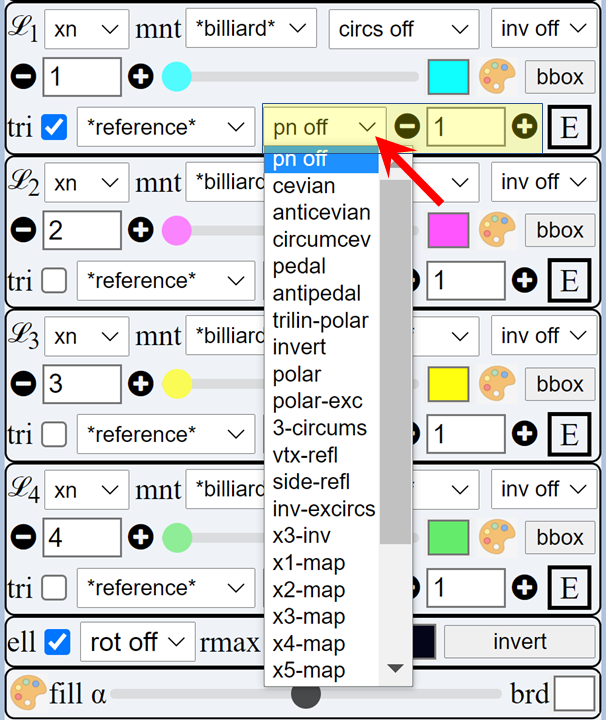
\includegraphics[width=.6\textwidth]{pics_09_090_cevian.png}
    \caption{Cevian-like triangles and number box to select a triangle center playing the role of $Q$ (see text).}
    \label{fig:09-menu-cevian}
\end{figure}

\subsection{Traditional}

Available in this groups are the standard constructions for (i) Cevian,  (ii) Anticevian, (iii) Circumcevian, (iv) Pedal, (v) Antipedal, and (vi) Trilinear Polar triangles described in \cite{mw}. Recall that the latter produces a degenerate (segment-like) triangle, see \cite[Trilinear Polar]{mw}.

\subsection{Inversive}

\begin{itemize}
\item \texttt{invert}: $T_m$ will have vertices at inversions of the parent one with respect to a unit circle centered on $X_m$.
\item \texttt{polar}: $T_m$ will be bounded by the polars (infinite lines) of the parent's vertices with respect to a unit circle centered on $X_m$, see \cite[Polar]{mw}.
\item \texttt{inv-excircs}: $T_m$ will have vertices at inversions of $X_m$ with respect to its excircles, see \cite[Excircle]{mw}. 
\item \texttt{polar-exc}: $T_m$ will be bounded by the polars (infinite lines) of $X_m$ with respect to each of the parent's excircles. 
\end{itemize}


\subsection{Reflexive}

\begin{itemize}
\item \texttt{vtx-refl}: $T_m$ has vertices at the reflections of $X_m$ on the parent vertices. 
\item \texttt{side-refl}: $T_m$ has vertices at the reflections of $X_m$ on the sidelines of the parent triangle.
\end{itemize}

\subsection{Triangulated}

Triangulate the parent with respect to $X_m$, i.e., consider the following subtriangles: $T_{23} = X_m P_2 P_3$, $T_{31} = X_m P_3 P_1$, and $T_{12} = X_m P_1 P_2$.

\begin{itemize}
\item \texttt{3-circums}: $T_m$ has vertices at the circumcenters of $T_{23}$, $T_{31}$, and $T_{12}$. 
\item \texttt{3-inv}: The inverse of \texttt{3-circums}. $T_m$ is such that the circumcenters of its three sub-triangles are the vertices of the parent. The vertices of $T_m$ are the non-$X_m$ intersections of a circle through $X_m$ and $P_i$ with a circle through $X_m$ and $P_{i+1}$, cyclically. 
\item $X_k$-map, $k\in[1,11]$: $T_m$ has vertices at the $X_k$ of $T_{23}$, $T_{31}$, and $T_{12}$. Note: $X_3$-map is the same as the \texttt{3-circums} setting.
\end{itemize}
